\chapter{Verwandte Arbeiten}
\label{chap:relatedwork}
Dieses Kapitel behandelt verwandte Arbeiten, die bis in das Jahr 1998 zurückreichen. Im November 1998 veröffentlichten Schmidt et al. im Rahmen des \textit{Technology for Enabling Awareness (TEA)}-Projektes ein Paper über \textit{Context Awareness in Ultra-Mobile Computing}, in dem sie darauf hinwiesen, dass Kontext mehr beinhaltet als den Ort des Geschehens, auf den sich vorige Werke konzentrierten \cite{Schmidt1999}. In diesem Paper schlugen sie neben der Verwendung expliziter Regeln zur Erkennung diverser Aktivitäten zusätzlich auch die Verwendung von Methoden künstlicher Intelligenz vor.

Parallel dazu erkannte Ashbrook 1999 ebenfalls die Bedeutung der Kontexterkennung als wichtige Komponente tragbarer Computeranwendungen \cite{Ashbrook1999}. Ein damals kommerziell verfügbares Produkt namens \textit{Twiddler}, eine mit nur einer Hand bedienbare Tastatur, integrierte zwei Sensoren, welche die Ausrichtung des Gerätes feststellen konnten. Mit der Motivation, automatisch eine To-Do-Liste zu öffnen, wenn der Nutzer des Gerätes sich zu seinem nächsten Termin bewegt, untersuchte Ashbrook die Möglichkeit, eben diese Tätigkeit mithilfe der genannten Sensoren automatisch erkennen zu lassen. Er schlug mehrere solche Methoden vor, die allerdings allesamt keinen Gebrauch von Machine Learning machten und nur schwer auf andere Aktivitäten übertragbar waren.

Ebenfalls im Jahr 1999 äußerten Farringdon et al. Kritik an Mobilgeräten wie Handys und PDAs, die ihre Besitzer auch in unangemessenen Situationen visuell und akustisch über eingehende Nachrichten benachrichtigen \cite{Farringdon1999}. Um dieses Problem anzugehen entwickelten sie ein an der Hüfte tragbares Gerät, das zwei 1D-Accelerometer integrierte, sowie eine Jacke, die den Streckfaktor des Materials messen konnte. Auch hier wurde Machine Learning nicht eingesetzt. Stattdessen wurde für die Erkennung der Aktivitäten Sitzen, Stehen, Liegen, Gehen und Laufen ein Algorithmus entwickelt, der Aspekte wie die Durchschnittswerte der Sensoren betrachtet und mit Schwellwerten vergleicht.

\begin{figure}
\centering
\includegraphics[clip,trim=25mm 90mm 110mm 115mm, page=6, scale=1]{img/VanLaerhoven2000}
\caption{Der Aufnahmeprozess von Van Learhoven und Cakmakci \cite{VanLaerhoven2000}}
\label{fig:van-laerhoven-experiment}
\end{figure}

Das TEA-Projekt wurde über mehrere Jahre fortgeführt. Nach den Publikationen von Ashbrook und Farringdon et al. wurde im Rahmen dieses Projektes 2000 ein Paper von Van Learhoven und Cakmakci veröffentlicht, das unter anderem die Arbeit von Ashbrook anerkannte, jedoch darauf hinwies, dass Kontexterkennung adaptiv sein muss und sich dafür Methoden des maschinellen Lernens anbieten \cite{VanLaerhoven2000}. Als mindestens eines der ersten Werke zu diesem Thema setzen die Autoren mehrere Sensortypen ein und verwenden neben Beschleunigungssensoren auch Infrarot-, Temperatur-, Kohlenstoffmonoxid-, Berührungs- Druck- und Lichtsensoren sowie Mikrofone, die in einem am Oberschenkel tragbaren Gerät integriert wurden. 
Diese Fülle von Daten verursachte zu diesem Zeitpunkt noch Probleme hinsichtlich des Rechenaufwands, weshalb die Autoren diverse Vorverarbeitungstechniken wie beispielsweise eine Fouriertransformation einsetzten, um die Datenmenge zu reduzieren. Anschließend verwendeten sie eine \textit{Kohonne Self-Organizing Map (KSOM)} als neuronenbasiertes Clusteringverfahren, in dem verschiedene Eingabewerte nach dem Trainingsprozess verschiedene Neuronenareale aktivieren. Dies ermöglichte eine Visualisierung des Clusterings und ließ die Autoren darauf schließen, dass eine Erkennung von Aktivitäten mithilfe von Machine Learning grundsätzlich möglich ist. Auf Basis der KSOM arbeitete anschließend ein $k$NN-Verfahren: Für einen Teil der Neuronen war bekannt, welche Aktivität sie aktiviert, sodass für die aktivierten Neuronen für eine Eingabe die $k$ nächsten Nachbarn dieser Neuronen für eine Abstimmung über die Aktivität betrachtet werden konnten. Dieses Verfahren, das auf einem Notebook in Echtzeit arbeitete, lieferte für die Aktivitäten Sitzen, Stehen, Gehen, Laufen und Fahrradfahren gute Ergebnisse, nur das Treppensteigen sorgte für Probleme. Abbildung~\ref{fig:van-laerhoven-experiment} zeigt die Einschränkungen des Experiments durch die beschränkte Rechenleistung und Speicherkapazität der zum Zeitpunkt der Arbeit verfügbaren mobilen Technologie.

Nicht nur im Sinne der \textit{Context Awareness} gab es Entwicklungen im Bereich der Aktivitätenerkennung. Auch für medizinische Zwecke hat diese Technologie Relevanz, beispielsweise bei Rehabilitationstherapien. 2001 veröffentlichten Bussmann et al. ein Paper über den sogenannten \textit{Activity Monitor}, der für diesen Zweck entwickelt wurde \cite{Bussmann2001}. Um die Aktivitäten Liegen, Sitzen, Stehen, Gehen, Laufen, Treppensteigen, Fahrradfahren, Rollstuhlfahren und Übergänge dazwischen erkennen zu können, wurde ein tragbares Gerät entwickelt, das Sensordaten aufzeichnet. An mehreren Körperstellen wurden Sensoren befestigt, die kabelgebunden Daten an einen Rekorder übermittelten, der in einem Beutel an der Hüfte des Trägers angebracht wurde. Aus den Rohdaten wurden Features extrahiert, die allerdings nicht für das Training eines ML-Algorithmus eingesetzt wurden, sondern für die manuelle Erstellung einer Datenbank zur Erkennung der Aktivität. Dafür wurden für die extrahierten Features pro Aktivität Minima und Maxima definiert, sodass die summierte Distanz der Eingabefeatures von diesen Intervallen zur Klassifikation berechnet werden konnte. Dieser manuelle Prozess ermöglichte in vier Studien Übereinstimmungen der Klassifikation mit den tatsächlichen Aktivitäten von $89 \%, 93 \%, 81 \%$ und $90 \%$. Eine große Schwäche des Gesamtkonzepts war die Größe des Activity Monitors, durch die Aktivitäten beeinflusst oder sogar vollständig verhindert wurden. Ein weiteres Problem waren die mit 10000 USD angegebenen Kosten des Gerätes. Dank der heutigen Technik wurden diese Probleme weitgehend eliminiert, jedoch verbleibt ein ethisches Problem, das die Autoren erkannten: Der Monitor könnte als \textit{Big Brother} aufgefasst werden, der die Privatsphäre des Benutzers einschränkt. Insbesondere im sensiblen medizinischen Kontext trifft dies zu.

Bao und Intille prüften im Jahre 2004 in einer Studie mit 20 Teilnehmern und Aktivitäten, ob Aktivitätenerkennung auch außerhalb von Laborbedingungen praktikabel ist, da sie vermuteten, dass sich Menschen im Labor anders verhalten als im alltäglichen Leben. Des Weiteren wurden zur größeren Bewegungsfreiheit diverse am Körper installierte Sensoren nicht mit einem zentralen Rekorder verbunden, sodass jeder Sensor separate Aufnahmen erzeugen musste. Dies warf wie in dieser Arbeit die Frage auf, inwiefern Abweichungen der Uhren der Aufnahmegeräte zum Problem werden könnten, weshalb man sich zu einer Synchronisierung zum Start und Ende der Aufnahme entschlossen hat.
Um möglichst realitätsnahe Aufnahmen zu erzeugen, entwickelten Bao und Intille einen Parcours mit Aufgabenstellungen, die die aufzunehmenden Aktivitäten beinhalteten, jedoch nicht als Hauptziel hatten. Die Teilnehmer des Experiments wurden dabei nicht beobachtet und mussten selbst notieren, wann sie eine Aufgabe angefangen und abgeschlossen hatten. Einige Aktivitäten wurden außerhalb eines Labors aufgenommen. Auf Basis dieser Daten wurden mithilfe von ML-Klassifikationsalgorithmen Modelle trainiert und ausgewertet. Mit einer Genauigkeitsrate von etwa $85 \%$ waren die Ergebnisse für Modelle, die keine nutzerspezifischen Informationen beinhalteten, vergleichbar mit Ergebnissen, die in anderen Werken unter Laborbedingungen erzeugt wurden. Dies deutet darauf hin, dass ein aufwendiger Parcours nicht unbedingt notwendig ist, um aussagekräftige Ergebnisse zu erhalten.
Eine weitere interessante Erkenntnis von Bao und Intille war, dass ein Beschleunigungssensor am Oberschenkel die größte Aussagekraft hatte und dass ein Beschleunigungssensor am dominanten Arm des Trägers nützlicher war als am nichtdominanten Arm. Die zweitgrößte Aussagekraft hatte ein Sensor an der Hüfte des Trägers, woraus die Autoren schlossen, dass ein am Handy angebrachter Sensor ähnliche Ergebnisse erzielen könnte. Dies deutet auf gute Voraussetzungen für meine Methode hin, in der Daten von einem Smartphone in der Hosentasche und von einem Fitness-Tracker am dominanten Arm aufgenommen werden.

2005 untersuchten Ravi et al. mit einem via Bluetooth verbundenen Beschleunigungssensor unter anderem, welche Features im Kontext der Aktivitätenerkennung sinnvoll und welche Aktivitäten besonders schwer zu erkennen sind \cite{Ravi2005}. Eines der getesteten Features war die sogenannte \textit{Energie} als Summe der Komponenten, die aus einer Fouriertransformation der sequentiellen Daten hervorging. Da eine Fouriertransformation diese in ein Frequenzspektrum zerlegt, erhofften sich die Autoren in diesem Feature die Periodizität der Aktivitäten widerspiegeln zu können, jedoch erwies sich dieses Feature nicht als signifikant. Wie Bao und Intille stellten auch die Autoren dieser Arbeit fest, dass ein Beschleunigungssensor auf Hüfthöhe Aktivitäten gut erkennen kann, jedoch bei handorientierten Aktivitäten Schwächen zeigt.

Thematisch anknüpfend an die bereits 2004 gewonnenen Erkenntnisse von Bao und Intille veröffentlichten Kwapisz, Weiss und Moore 2010 ein Paper, das erfolgreiche ML-basierte Aktivitätenerkennung auf einer Datenbasis demonstrierte, die exklusiv mithilfe von Smartphone-Beschleunigungsensoren gewonnen wurde. Die Arbeit der Autoren lieferte die Grundlage für den in Abschnitt~\ref{sec:transformation} dieser Arbeit beschriebenen Transformationsprozess \cite{Kwapisz2012}. 2012 untersuchten Weiss und Lockhart auf Basis dieser Methode, inwiefern die Personalisierung von Modellen durch nutzerspezifische Aufnahmen diese verbessert und kamen zu dem Schluss, dass eine Personalisierung die Genauigkeit bedeutend verbessert. 2016 verwendeten Weiss et al. statt eines Smartphones erfolgreich eine Smartwatch und demonstrierten insbesondere für handorientierte Aktivitäten starke Verbesserungen der Klassifikationsgenauigkeit \cite{Weiss2016}.

Die Kombination mehrerer Smartphone-Sensoren wurde 2012 erstmals von Suarez et al. durchgeführt und demonstrierte, dass damit eine Verbesserung der Genauigkeit um $10 \%$ und mehr möglich ist \cite{Dernbach2012}.

Meines besten Wissens nach ist diese Arbeit somit die erste, in der die Daten mehrerer Sensoren eines Smartphones mit den Daten mehrerer Sensoren eines Fitness-Trackers kombiniert werden, der mehr Sensoren als eine reguläre Smartwatch besitzt.

% vim: set ft=tex
